\subsection{Detection}

\subsubsection{Introduction \& Motivation}

%{\bf Input from John.}

Deep neural networks are ubiquitous within image classification problems, often exhibiting greater classification accuracy relative to alternative methods. This can be attributed to the multilayer structure of deep networks, the convolutional layers . However, deep networks have been shown (reference?) to be sensitive to slight changes in the input data, often resulting in incorrect classification. This is arguably an inherent feature of deep neural network, given the very non-convex nature of the prediction function represented by the network. Adversarial attacks (DEFINED ELSEWHERE IN REPORT?) exploit this vulnerability of deep neural networks to e.g. bypass security systems. We thus examine the problem of detecting adversarial attacks, focusing on a simple class known as  fast-gradient sign method (FGSM - REFERENCE!!!!) adversarial attacks.

\subsubsection{Problem Set-up}\label{Setup}

FGSM attacks are constructed by perturbing a non-adversarial image with a fixed level of noise $\varepsilon \in \mathbb{R}$ up to the sign of the loss function $L$ with respect to the feature space $x$:
\begin{equation}
\mathbf{\tilde{X}}=\mathbf{X} + \text{sign}{\nabla_x L(\theta,\mathbf{X},y)}\cdot\varepsilon,
\end{equation}
where $\mathbf{X} \in \mathbb{R}^n$ is the flattened image and $y$ is the true class label. $\varepsilon$ is chosen to be sufficiently small to make detection of image tampering invisible to the human eye, but sufficiently large to induce an incorrect classification by the neural network. Given the nature of the perturbation, it is clear that this class of attack is available to attackers only if they have access to the analytic form of the loss function associated with the neural network they are attacking. 

\par 

We consider identifying FGSM attacks for a network a four-layer network consisting of two convolutional layers followed by two fully-connected layers. The first convolutional layer takes as input a one-channel, $28\times 28$ image and outputs five channels based on a $5\times 5$ kernel. The second layer outputs 20 channels, also based on a $5\times 5$ kernel, with randomly-selected dropouts. We apply max-pooling to $2\times 2$ grids of the output of each convolutional layer. The first fully-connected layer takes as input a vector $\in \mathbb{R}^{320}$ and outputs in $\mathbb{R}^{50}$, before applying a ReLu activation function to this output. The final layer uses a log-softmax function to output the classification probabilities. We consider the MNIST dataset; thus the output of the final layer is $\in [0,1]^{10}$.

\subsubsection{Approach}

We trained the neural network described in Section \ref{Setup} on MNIST training data, containing 60,000 examples of handwritten digits in 0-9.  Using the FGSM approach with $\varepsilon =\{0.05,0.1,0.15,0.2,0.25,0.3\}$ we find about 45,000 successful adversarial examples for our network and data set.
\par
We next choose a subset of 8,000 images from the training set and pass these through the net, obtaining the vectorised features $\boldsymbol{\phi}_{j}$ from each layer $j=\overline{1,4}$. We then train a linear PCA dimensionality reduction model $M_j$ for each layer using these $\boldsymbol{\phi}_j$. For each layer, we keep the first $n_j$ principal components such that we retain approximately 90\% of the variance in the data. This gives $(n_1, n_2, n_3, n_4) = (75, 55, 12, 12)$. We show in Figure \ref{fig:PCA} the fractional variance and cumulative variance captured by each principal component for each layer.

\begin{figure}
\centering
\begin{subfigure}{.5\textwidth}
  \centering
  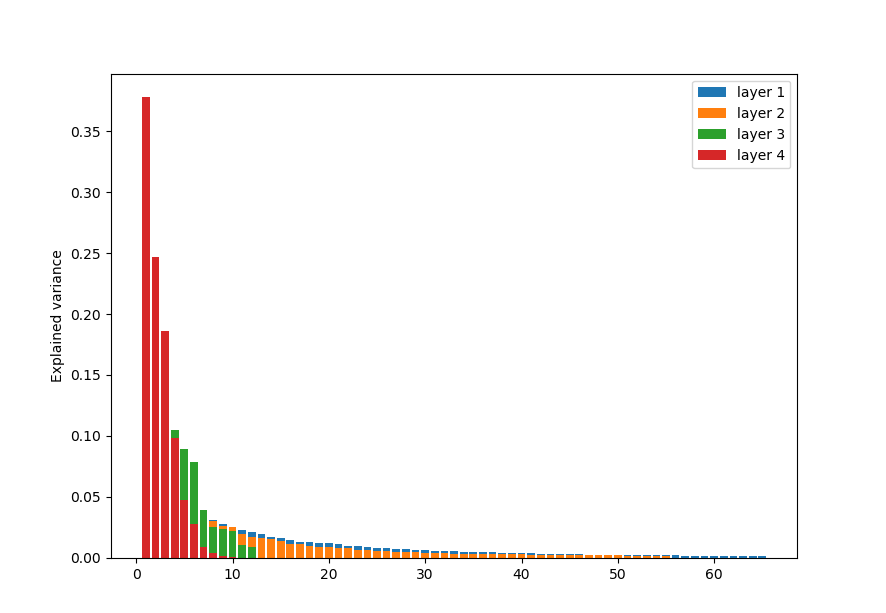
\includegraphics[width=.6\linewidth]{ExplainedVarianceLegend.png}
  \caption{Explained variance of principal components}
  \label{fig:PCA1}
\end{subfigure}%
\begin{subfigure}{.5\textwidth}
  \centering
  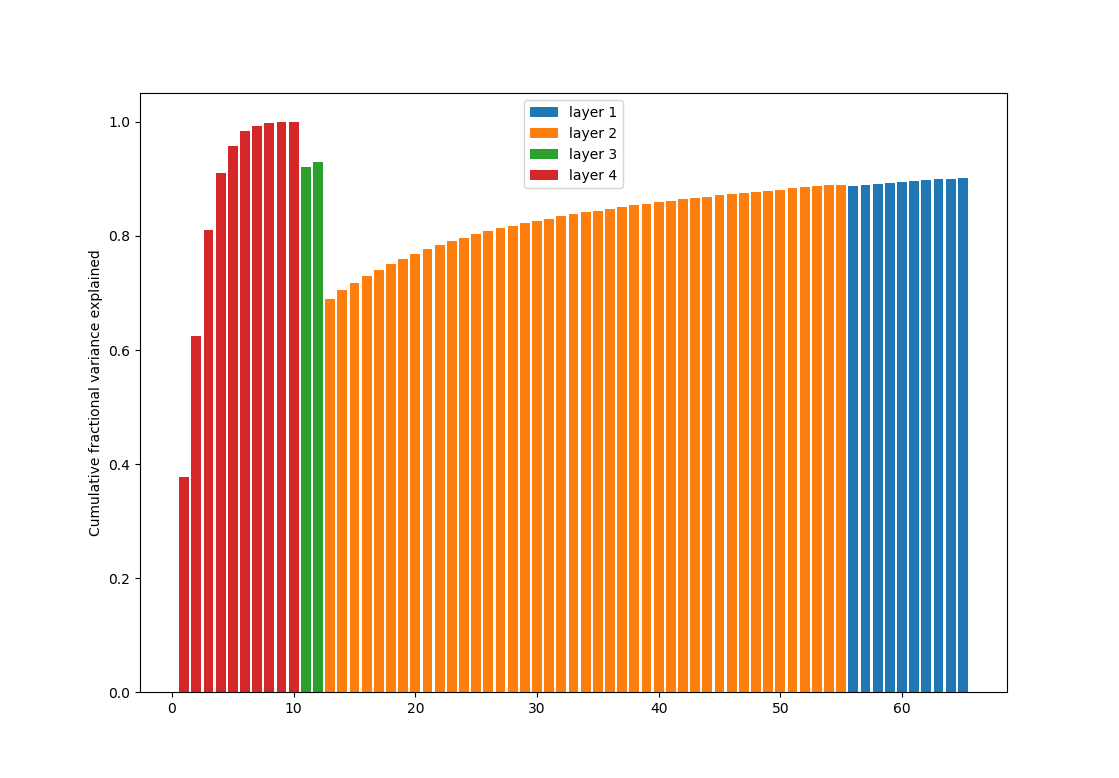
\includegraphics[width=.4\linewidth]{CumExplainedVarianceLegend.png}
  \caption{Cumulative explained variance of principal components}
  \label{fig:PCA2}
\end{subfigure}
\caption{}
\label{fig:PCA}
\end{figure}
Note that this does not require access to the adversarial attacks. For each layer we next train a k-nearest neighbour model on the uncorrupted data, with $k=20$, and using the reduced dimension space found with PCA. For all the test examples we will thus find the closest 20 neighbours from the training data, and the corresponding distances.  We use this to compute the Local intrinsic dimensionality (LID) (REFERENCE NEEDED) for each data point, in each layer. Thus, each data sample is now characterised by $\mathbf{l}_i \in \mathbb{R}^4$, corresponding to the four layers. We consider the practical approximation of LID, defined as (REFERENCE)
\begin{equation}
LID(x) = -\left(\frac{1}{k}\sum_{i=1}^{k}\log\frac{r_i(x)}{r_k(x)}\right)^{-1},
\end{equation}
where $r_i(x)$ denotes the distance between $x$ and its $i$ nearest neighbour within the 8,000 uncorrupted data points, and $r_k(x)$ is the maximum of these values. Note that in our case $x$ corresponds to the reduced feature vector of each datapoint, for each layer.

We next randomly choose a subset of about 8,000 successful adversarial examples, together with the training set. We train a classifier $\mathcal{C}$ that takes as input for each data point the LID vector $\mathbf{l}_i$ and outputs $y=1$ if the example is adversarial and $0$ otherwise. We consider Logistic Regression and SVM for $\mathcal{C}$.